
\documentclass[10pt,twocolumn,a4paper]{article}

% --- PACKAGES ---
\usepackage[utf8]{inputenc}
\usepackage[top=0.45in, bottom=0.55in, left=0.55in, right=0.55in]{geometry}
\usepackage{amsmath,amssymb,amsfonts}
\usepackage{booktabs}
\usepackage{graphicx}
\usepackage{hyperref}
\usepackage{enumitem}
\usepackage{microtype}
\usepackage{xcolor}
\usepackage{titlesec}

% --- COLUMN & TABLE STYLING ---
\setlength{\columnsep}{18pt}
\setlength{\heavyrulewidth}{0.4pt}
\setlength{\lightrulewidth}{0.25pt}

% --- SECTION STYLING & SPACING ---
\titleformat{\section}{\large\bfseries}{\thesection.}{0.4em}{}
\titleformat{\subsection}{\normalsize\bfseries}{\thesubsection}{0.4em}{}
\titlespacing*{\section}{0pt}{5pt}{2pt}
\titlespacing*{\subsection}{0pt}{4pt}{2pt}

\hypersetup{
    colorlinks=true,
    linkcolor=blue,
    citecolor=blue,
    urlcolor=blue
}

% --- TITLE & AUTHOR INFO ---
\title{\vspace{-1.2em}\textbf{\Large %Computational Formalization and Reinforcement Learning Baselines for Assamese Traditional Games: A Case Study on Kori Khel
KoriKhelEnv: A Gymnasium Reinforcement Learning Environment and Associated Experimentation for a Traditional Assamese Game}\vspace{-0.4em}}

\author{
    \textbf{Dipjyoti Das}\textsuperscript{1}, \textbf{Simanta Sarma}\textsuperscript{1}, \textbf{Rupam Bhattacharyya}\textsuperscript{1} \\
    \textsuperscript{1}Responsible Bot Lab, Department of Information Technology, Gauhati University, Assam, India
}

\date{\vspace{-2.0em}}

\begin{document}

\maketitle

% --- ABSTRACT ---
\begin{abstract}
Digital representation of India’s traditional games should be encouraged to demonstrate the richness of Indian culture. Reinforcement Learning (RL) benchmark environments have focused primarily on standardized Western board and video games. %Consequently, indigenous multi-agent board games featuring asymmetric stochastic dynamics and complex topological constraints remain largely unmodeled in standard RL benchmark suites. 
In this paper, we present a computational formalization and Gymnasium environment for \textbf{Kori Khel}, a traditional 4-player stochastic cowrie-shell board game native to Assam, India. We abstract the physical 2D cross-shaped board into a 73-state 1D Markov Decision Process (MDP) per player, incorporating asymmetric binomial dice distributions, 8 safe zones, and capture mechanics. We evaluate policy gradient baselines using Proximal Policy Optimization (PPO) under two regimes: standard reward-penalty shaping (2M timesteps) and invalid action masking (2M timesteps). Across a 1,000-game evaluation benchmark, Standard PPO fails to maintain legal play (88.4\% rule adherence, 28.90\% win rate) due to severe entry-state bottlenecks. In contrast, Maskable PPO achieves 100\% rule adherence, an average episode reward of +115.15, and a \textbf{38.10\% win rate} against rule-compliant opponents in a 4-player setting (outperforming the 25.0\% random baseline). %We analyze the mathematical necessity of action masking in stochastic games with hard entry constraints and outline directions toward formalizing broader suites of regional games.
\end{abstract}

\textbf{\small Keywords---} Reinforcement Learning, Proximal Policy Optimization, Action Masking, Traditional Game Formalization, Kori Khel.

% --- SECTION 1: INTRODUCTION ---
\section{Introduction}
\textbf{Kori Khel}\footnote{Figure 1 is adapted from https://itfc.assam.gov.in/} is a 4-player cowrie-shell race game played across rural Assam, India. Structurally resembling Pachisi and Ludo, it is characterized by a highly skewed binomial dice distribution and a strict entry constraint: tokens remain trapped off-board ($s=0$) until an exact roll (\textit{Jagowa}) is obtained. This entry rule induces a bottlenecked action space where reward-penalty shaping fails to guide unmasked policy gradient methods, rendering Kori Khel a compelling domain for evaluating invalid action masking techniques.

\begin{figure}[h]
\centering
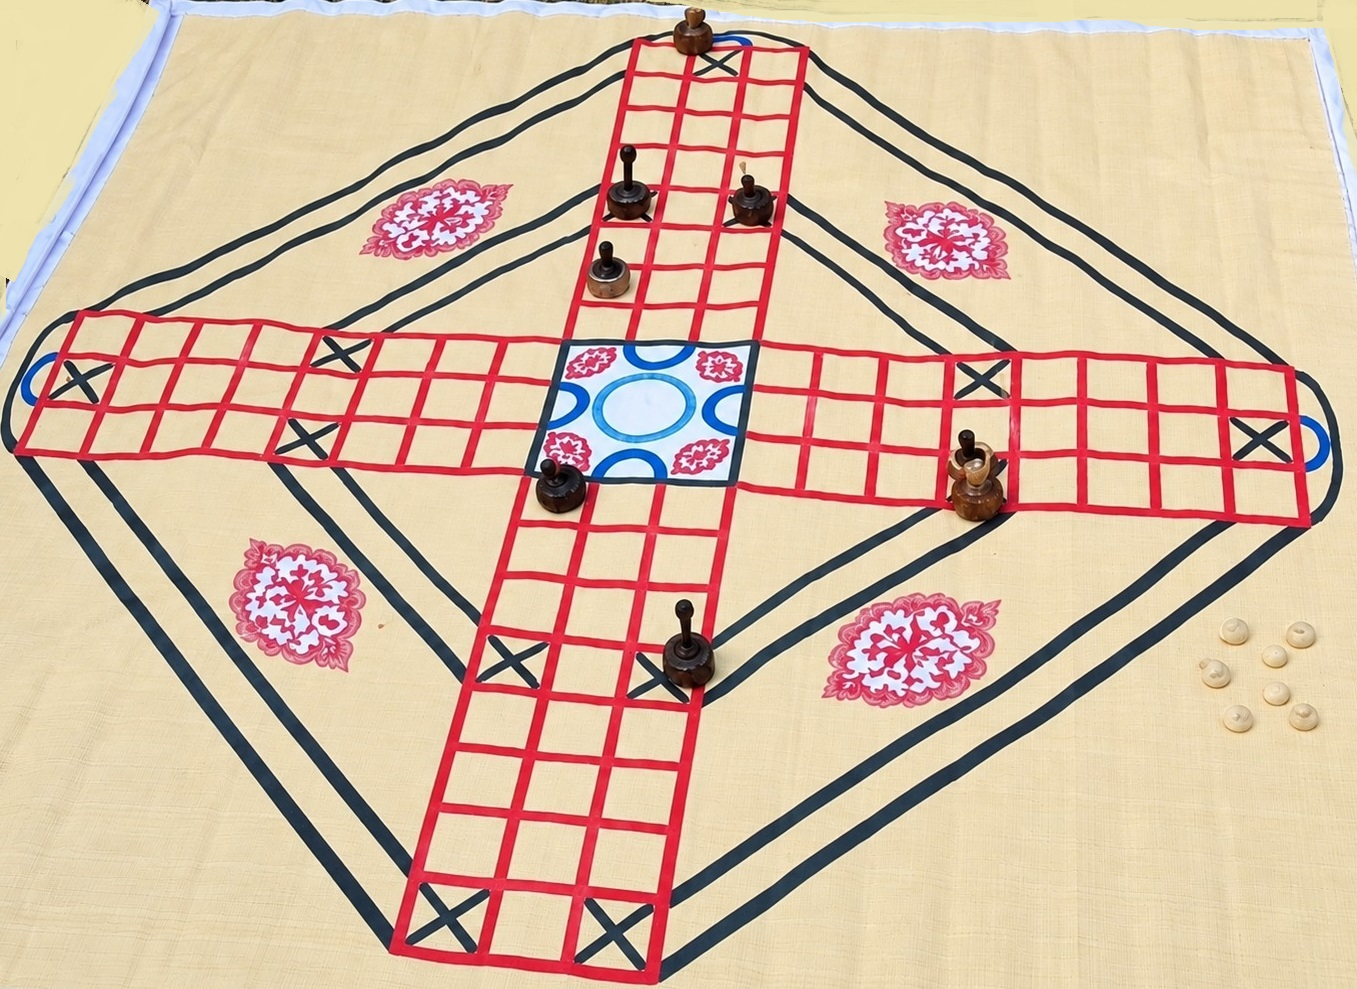
\includegraphics[width=1\linewidth]{koriboard.jpeg}
\caption{Visual representation of the board involved in kori khel}
\label{kori1}
\end{figure}

%While RL benchmark suites encompass Chess, Go, and StarCraft II, regional Indian games lack standardized computational state-space definitions. 
This work addresses this gap through the following contributions:
\begin{enumerate}[leftmargin=*,noitemsep,topsep=1pt]
    \item A formal state-space specification of Kori Khel, mapping its physical 2D cross grid into a 73-state 1D coordinate system.
    \item An open-source OpenAI Gymnasium environment \footnote{https://gymnasium.farama.org/index.html} (\texttt{KoriKhelEnv}).
    \item A comparative empirical benchmark evaluating Standard PPO versus Maskable PPO under stochastic dice conditions.
\end{enumerate}

% --- FIGURE 2: PLACED EARLY SO LATEX PUTS IT AT TOP OF PAGE 2 ---
\begin{figure*}[t]
\centering
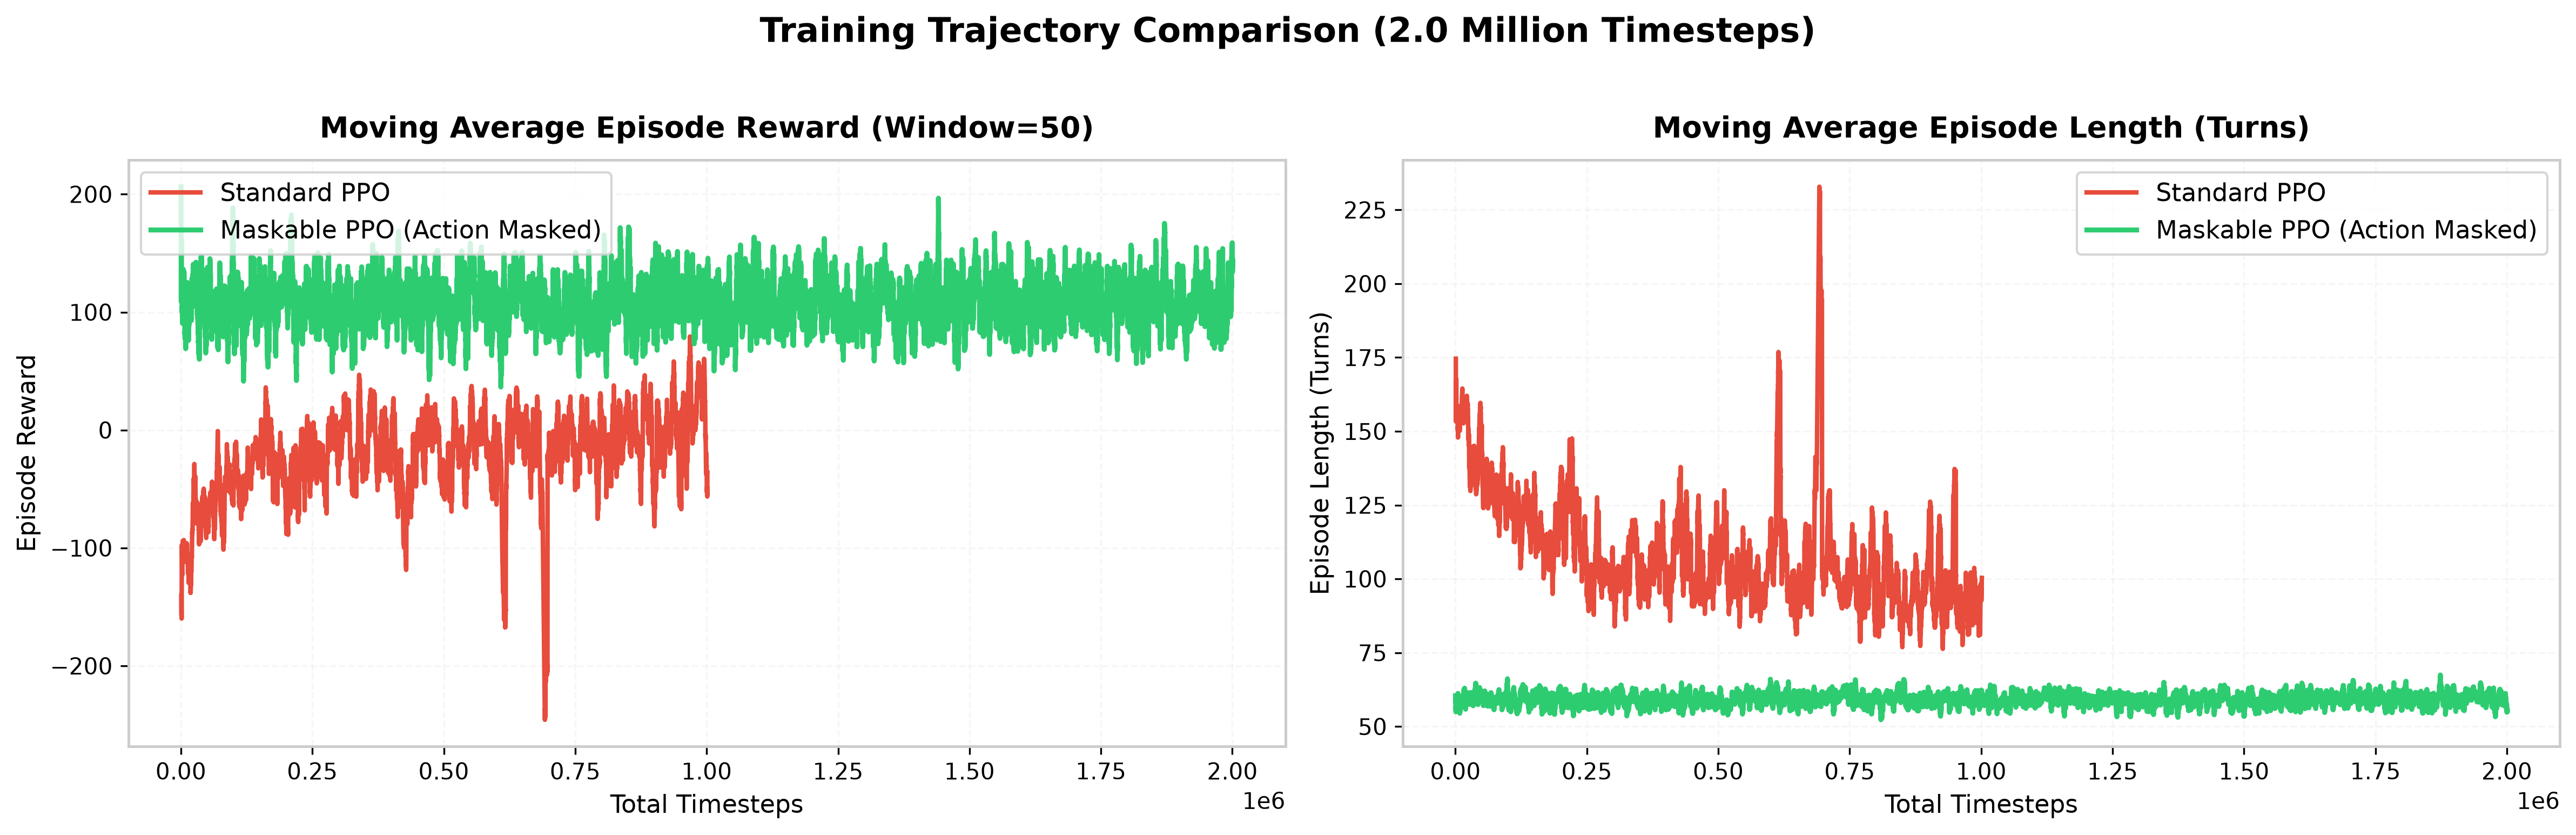
\includegraphics[width=1\textwidth]{../evaluation/kori_khel/plots/training_curves_comparison.png}
\caption{Training Trajectory Comparison over 2 million timesteps showing moving average reward and episode length convergence.}
\label{fig:learning_curves}
\end{figure*}

% --- SECTION 2: MATHEMATICAL FORMULATION ---
\section{Kori Khel Game Formalization}

\subsection{Asymmetric Stochastic Roll Model}
Kori Khel is played with 6 cowrie shells (\textit{kori}). The outcome of a throw is defined by the number of shells landing face-down (\textit{uburi}), modeled as a binomial variable $K \sim \text{Binomial}(6, p=0.5)$:
\begin{equation}
\mathbb{P}(K = k) = \binom{6}{k} (0.5)^6
\end{equation}
Certain throws in Kori Khel carry traditional terminology and grant special advantages, such as bonus turns or the mandatory board-entry condition:
\begin{itemize}[leftmargin=*,noitemsep,topsep=1pt]
    \item \textbf{Pochi ($k=5$, 1 Open, 5 Closed):} 25 steps + Bonus Turn ($\mathbb{P} \approx 9.38\%$).
    \item \textbf{Jagowa ($k=1$, 5 Open, 1 Closed):} 10 steps + Bonus Turn ($\mathbb{P} \approx 9.38\%$) --- \textit{Mandatory entry roll required to release tokens from Base.}
    \item \textbf{Mudra ($k=0$, 6 Open, 0 Closed):} 12 steps + Bonus Turn ($\mathbb{P} \approx 1.56\%$).
    \item \textbf{Standard Throws ($k \in \{2, 3, 4, 6\}$):} 4, 3, 2, 6 steps respectively (No bonus turn).
    \item \textbf{3-Blow Rule:} Rolling 3 consecutive bonus turns invalidates all accumulated points for that turn.
\end{itemize}

\subsection{Board Abstraction \& MDP Mapping}
The physical board consists of 4 arms arranged in a cross ($+$), each with 3 columns of 8 cells. We map this 2D geometry into a \textbf{1D state sequence of 73 positions} for each player:
\begin{itemize}[leftmargin=*,noitemsep,topsep=1pt]
    \item \textbf{State $s = 0$ (Base):} Token is inactive off-board; requires a \textit{Jagowa} (10) roll to enter state $1$.
    \item \textbf{States $s \in [1, 64]$ (Shared Outer Perimeter):} Shared 64-cell track traversed in a strict global counter-clockwise spiral across the 4 board arms. Collisions on non-safe cells result in capture (\textit{Khua}), returning the opponent to $0$.
    \item \textbf{Safe Zones ($X$ Marks):} 8 designated sanctuary cells (Row 4 outer cells on perimeter) where collisions do not trigger capture ($s \in \{5, 12, 21, 28, 37, 44, 53, 60\}$).
    \item \textbf{States $s \in [65, 72]$ (Private Home Corridor):} Private 8-cell central corridor leading to the center.
    \item \textbf{State $s = 73$ (Ghai / Goal):} Terminal winning state (\textit{Pokoa}). First player to move all 4 tokens to 73 wins.
\end{itemize}

% --- SECTION 3: RL ARCHITECTURE ---
\section{Reinforcement Learning Architecture}

\subsection{Observation \& Action Spaces}
\begin{itemize}[leftmargin=*,noitemsep,topsep=1pt]
    \item \textbf{Observation Vector $\mathbf{o} \in \mathbb{Z}^{30}$:} Concatenates raw positions and engineered tactical features: $[s_{0..3}, s^{\text{opp}}_{1..12}, r, b, \mathbf{c}_{0..3}, \mathbf{z}_{0..3}, \mathbf{d}_{0..3}]$, where $s_{0..3}$ denote active agent positions ($[0,73]$), $s^{\text{opp}}_{1..12}$ denote opponent positions across seats, $r \in [0,25]$ is the dice roll, $b \in \{0,1\}$ is the bonus turn flag, $\mathbf{c} \in \{0,1\}^4$ indicate projected captures, $\mathbf{z} \in \{0,1\}^4$ indicate safe-zone landings, and $\mathbf{d} \in [0,64]^4$ measure rear threat distances.
    \item \textbf{Action Space $a \in \{0, 1, 2, 3\}$:} Discrete action selecting which of the 4 agent tokens to advance.
\end{itemize}

\subsection{Reward Design \& Coefficient Justification}
\begin{equation}
\mathcal{R}(s, a, s') = r_{\text{progress}} + r_{\text{event}}
\end{equation}
where $r_{\text{progress}} = +0.1 \times (s' - s)$, $r_{\text{capture}} = +20$, $r_{\text{captured}} = -20$, $r_{\text{ghai}} = +30$, $r_{\text{win}} = +100$ ($r_{\text{loss}} = -100$), and $r_{\text{invalid}} = -2$ (Standard PPO only).

The magnitude of each reward coefficient is scaled relative to the terminal match outcome ($\pm 100$). The intermediate milestone of landing a single token in Ghai ($+30$) is weighted below game termination to encourage multi-token coordination. Opponent captures are balanced symmetrically ($\pm 20$) to model competitive tactical exchanges without distorting value estimations. Step progress ($+0.1$) is set an order of magnitude smaller to eliminate reward-shaping loops, while $r_{\text{invalid}} = -2$ penalizes illegal actions without destabilizing gradient updates.

% --- SECTION 4: EMPIRICAL EVALUATION ---
\section{Empirical Benchmarks \& Results}
We trained Standard PPO for \textbf{2M timesteps} and Maskable PPO for \textbf{2M timesteps} against 3 rule-compliant heuristic opponents:
\begin{enumerate}[leftmargin=*,noitemsep,topsep=1pt]
    \item \textbf{Standard PPO (Unmasked, 2M):} Relies on penalty shaping ($r_{\text{invalid}} = -2$) to learn valid moves.
    \item \textbf{Maskable PPO (Masked, 2M):} Employs invalid action masking with linear learning rate decay ($3 \times 10^{-4} \to 5 \times 10^{-5}$) and tuned entropy coefficient ($\text{ent\_coef}=0.005$) to restrict policy distribution $\pi(a|s)$ exclusively to legal actions.
\end{enumerate}

\begin{table}[h]
\centering
\caption{Head-to-head benchmark performance over 1,000 matches.}
\label{tab:results}
\small
\setlength{\tabcolsep}{5pt}
\begin{tabular}{@{} l c c @{}}
\toprule
\textbf{Metric} & \textbf{Standard PPO} & \textbf{Maskable PPO} \\
\midrule
Win Rate (\%) & 28.90\% & \textbf{38.10\%} \\
Rule Adherence (\%) & 88.40\% & \textbf{100.00\%} \\
Avg Episode Length & 53.0 turns & \textbf{59.3 turns} \\
Avg Episode Reward & +88.24 pts & \textbf{+115.15 pts} \\
\bottomrule
\end{tabular}
\end{table}

\begin{figure}[h]
\centering
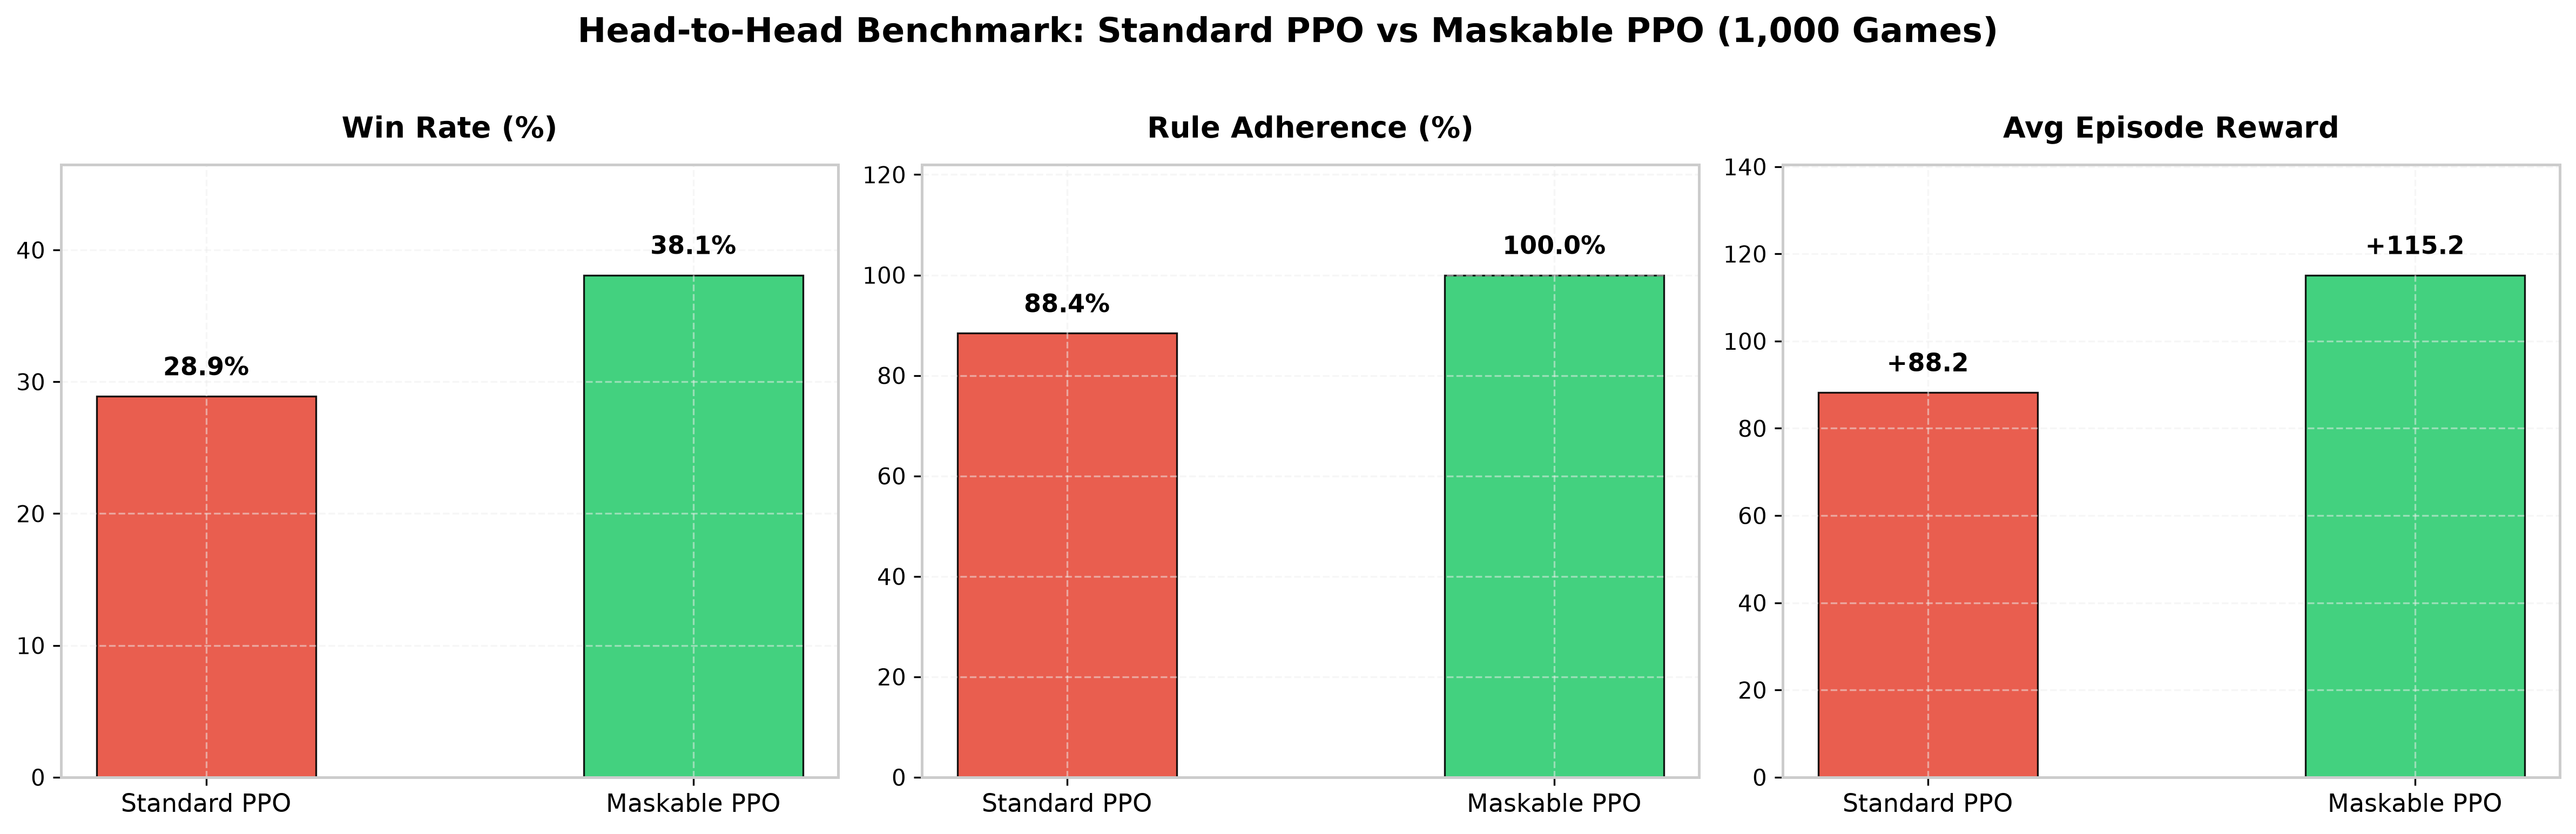
\includegraphics[width=1\linewidth]{../evaluation/kori_khel/plots/ppo_vs_maskable_comparison.png}
\caption{Head-to-Head 1,000-Game Benchmark Comparison across Win Rate (\%), Rule Adherence (\%), and Average Episode Reward (pts).}
\label{fig:benchmark_comparison}
\end{figure}

\subsection{Analytical Insights}
Standard PPO suffers from persistent invalid move sampling ($88.4\%$ rule adherence even after 2M steps). Because tokens at Base ($s=0$) require an exact roll of 10 to enter the board, unmasked agents repeatedly sample illegal actions, getting trapped in local penalty minima. Conversely, Maskable PPO guarantees 100\% legal play from step 1, achieving a \textbf{38.10\% win rate} after 2M steps that significantly outperforms the 4-player random baseline ($25.0\%$).

% --- SECTION 5: CONCLUSION & FUTURE WORK ---
\section{Conclusion}
This paper presented an MDP abstraction and Gymnasium benchmark environment for Kori Khel, proving that action masking is essential for overcoming entry-roll bottlenecks. According to our knowledge, this is the first work in the intersection of traditional Assamese games and RL. Having an open-source OpenAI Gymnasium environment for Kori khel is an important step towards representing Indian 
games in the modern RL-based game research. %Extending this framework to other regional games requires tailored state-space adaptations. In future, we would like to consider more traditional games across different states of India.
%Extending this framework to other regional games requires tailored state-space adaptations; for instance, formalizing \textbf{Dhop Khel} necessitates transitioning from our 73-state discrete single-track MDP to a continuous 2D spatial coordinate system with multi-agent ball-possession and tagging dynamics under partial observability.

% --- REFERENCES ---
\begin{thebibliography}{9}
\small
\setlength{\itemsep}{0.5pt}
\setlength{\parskip}{0pt}
\bibitem{ppo} J. Schulman et al., ``Proximal Policy Optimization Algorithms,'' \textit{arXiv:1707.06347}, 2017.
\iffalse
\bibitem{masking} S. Huang and S. Ontañón, ``A Closer Look at Invalid Action Masking in Policy Gradient Algorithms,'' \textit{FLAIRS Conference}, 2022.
\bibitem{gymnasium} M. Towers et al., ``Gymnasium: A Standard Interface for Reinforcement Learning Environments,'' \textit{arXiv:2407.17032}, 2024.
\fi 
\bibitem{nath2025evaluating}
R. Nath and R. Bhattacharyya,
``Evaluating Vision Language Models (VLMs) across six traditional games:
an evaluation paradigm to better assess culturally sensitive question answering systems,''
\textit{International Journal of Information Technology}, 2025.
doi:10.1007/s41870-025-02736-1.
\end{thebibliography}

\end{document}